%%% Started on  Fri Dec 15 16:03:20 2006 Roberto Cavada
%%% Last Sat Dec 16 18:15:11 2006 Roberto Cavada

\section{\label{DI}Details of implementation}
This section presents some details regarding the implementation of the
\mvco framework in Python.

\subsection{Models, Controllers and Views in detail}
The \mvco framework essentially supplies three base classes which
implement respectively a View, a Model and a Controller.  Developers
has to derive custom classes from the base classes set, adding the
implementation which depends on the application semantics.

\begin{description}

\item[Model base class] Supplies servicing for:
 \begin{itemize} 
 \item Fully automatic Observable Properties 
 \item Automatic broadcast notification when observable properties
 change.
 \item Transparent notifications to observers running in the \pygtk
   loop, even when sent by models running from other threads.
 \end{itemize}

\item[Controller base class] Supplies servicing for:
 \begin{itemize} 
 \item Automatic registration as observers of the associated Model.
 \item Easy access to the associated Model and View for any derived
 class.
 \end{itemize}

\item[View base class] Supplies servicing for:
 \begin{itemize} 
 \item Automatic widgets tree registration. Input can be a set of root
 widgets stored inside a \glade File, or a completely customized widgets
 hierarchies.
 \item Automatic registration inside the associated Controller.
 \item Automatic signals connection to methods supplied by the
 associated Controller.
\item Widget retrieval inside the set of hierarchy. Widget can be
  accessed by using the name they have been defined from within
  \glade, at design time, or that have been specified when creating
  widgets by hand.
\item (New in version 1.0.1) Support for custom widgets declared in
  \glade files.
 \end{itemize}

\end{description}


\subsection{\label{MODELS} Models}
Models must be used to hold the \emph{data} of the application. They
can be connected to observers (like Controllers) by a mechanism
detailed by section \ref{OPD}.  It is important to note that apart
from during the registration phase, the model do not know that there
exists a set observers connected to it.

All the code strictly related to the data of the application (i.e. not
related to any view of those data) will live in the model class. 

There exist several model classes that users can derive their own
classes:

\begin {description}
\item [gtkmvc.Model] Standard model class. The derived class does not
  multiple-derive from gobject classes, and there are not methods in
  the class that run from threads different from the \pygtk main loop
  thread. This is the base model class most likely users will derive
  their own models.

\item [gtkmvc.ModelMT] Multi-threading model used as the previous
  class Model, but to be used in all cases when the \pygtk main loop
  runs in a thread that is different from the thread running the
  model. This is the typical case of a model that needs to perform
  asynchronous operations that requires much time to complete, and
  that can be ran on a different thread making the \gui still
  responsive to the user actions. When the model's thread changes an
  observable property, corresponding notifications will be
  transparently delivered to the observers through their own thread.

\item [gtkmvc.TreeStoreModel] To be used as a base model class that
  derives both from \codename{Model} and \codename{gtk.TreeStore}.

\item [gtkmvc.TreeStoreModelMT] To be used as a base model class that
  derives both from \codename{ModelMT} and \codename{gtk.TreeStore}.

\item [gtkmvc.ListStoreModel] To be used as a base model class that
  derives both from \codename{Model} and \codename{gtk.ListStore}.

\item [gtkmvc.ListStoreModelMT] To be used as a base model class that
  derives both from \codename{ModelMT} and \codename{gtk.ListStore}. 

\item [gtkmvc.TextBufferModel] To be used as a base model class that
  derives both from \codename{Model} and \codename{gtk.TextBuffer}.

\item [gtkmvc.TextBufferModelMT] To be used as a base model class that
  derives both from \codename{ModelMT} and \codename{gtk.TextBuffer}.

\end{description}


\subsection{Controllers}
User's controllers must derive from this class.  A controller is
always associated with one model, that the controller can monitor and
modify. At the other side the controller can control a View.  Two
members called \codename{model} and \codename{view} holds the
corresponding instances.

The controller holds all the code that lives between data in model and
the data-presentation in the view. For example the controller will
read a property value from the model, and will send that value to the
view, to visualize it.  If the property in the model is an Observable
Property that the Controller is interested in monitoring, than when
somebody will change the property, the controller will be notified and
will update the view.


\subsubsection{Model registration}
By default, a controller is also an Observer (see below) of the
corresponding Model, even when there is nothing to observe, or when
the controller is interested in observing nothing within the model.

Registration occurs automatically. If the observation is not wanted,
the derived controller can call method
\codename{Model.unregister\_observer} from the instance constructor, to
unregister itself.


\subsubsection{\label{VR:D}View registration}
View registration (see View class, below) occurs during View
construction. An important method of the class Controller that user
can override is \codename{register\_view}, that the associated view
will call during registration. This can be used to connect custom
signals to widgets of the view, or to perform some initialization that
can be performed only when model, controller and view are actually
connected.  \codename{register\_view} gets the view instance that is
performing its registration within the controller. See section
\ref{VR:EX} for an example of how this mechanism may be exploited
effectively. 

\subsection{Views}
User's views derive from base class \codename{gtkmvc.View}, that is
the only part specific for the \pygtk graphic toolkit.

A View is always associated to a Controller. When the view is created,
it registers itself to the controller by calling method
\codename{Controller.register\_view}.

A View is also associated to a set of widgets. In general, this set
can be organized as a set of trees of widgets. Each tree can be
optionally be generated by using the \glade application 
(see section \ref{GLEX}). 


\subsubsection{Constructor}

The View constructor is quite much complicated:

{ \codesize 
\begin{verbatim} 
def __init__(self, controller, glade_filename=None,
             glade_top_widget_name=None, parent_view=None, 
             register=True)
\end{verbatim}} 


\begin{description}
\item[glade\_filename] can be either a string or a list of strings. In
  any case each provided string represents the file name of a \glade
  file. Typically each glade file contains a tree of (named) widgets.

\item[glade\_top\_widget\_name] can be a string or a list of strings.
  Each string provided is associated to the parameter glade\_filename
  content, and represent the name of the widget in the widgets tree
  hierarchy to be considered as top level. This let the user to select
  single parts of the glade trees passed through parameter
  \codename{glade\_filename}.

\item[parent\_view] is the view instance to be considered parent of
self. Generally this parameter is None. 

\item[register] is a flag used to delay view's registration to the
  controller. If your derived view class adds some widgets
  ``manually'' by creating them on the fly (see \ref{VIEW:MANUAL}),
  you want to delay the view registration until all widgets have been
  actually created.  Since the View's constructor must be called at
  the beginning of your derived view class constructor, you can avoid
  the View constructor calling \codename{Controller.register\_view} by
  setting this flag to \codename{False}. After user's view class
  constructor has built all the widgets, it is responsible for
  calling \codename{Controller.register\_view} to perform the
  registration.  (This is definitely more complicated to explain than
  to understand...  examples show how delayed registration can be
  used.)
\end{description}


\subsubsection{\label{VIEW:MANUAL}A widgets container}

The \codename{View} class can also be considered a map, that
associates widget names to the corresponding widget objects. If file
\file{test.glade} contains a Button that you called
\codename{start\_button} from within \glade, you can create the view
and use it as follows:

{ \codesize 
\begin{verbatim}
from gtkmvc import View

class MyView (View):
  def __init__(self, controller):
    View.__init__(self, controller, 'test.glade')
    return
  pass 

m = MyModel()
c = MyController(m)
v = MyView(c)

v['start_button'] # this returns a gtk.Button object
\end{verbatim}
}

Instead of using only \glade files, sometimes the derived views create
a set of widgets on the fly. If these widgets must be accessed later,
they can be associated simply by (continuing the code above):

{ \codesize 
\begin{verbatim}
v['vbox_widget'] = gtk.VBox()
...
\end{verbatim}
}

Typically the creation on the fly of new widgets is performed by the
derived view constructor, that will delay the view registration.

{ \codesize 
\begin{verbatim}
from gtkmvc import View

class MyView (View):
  def __init__(self, controller):
    View.__init__(self, controller, 'test.glade', register=False)
 
    # ad-hoc widgets
    v['vbox_widget'] = gtk.VBox()
    ...

    controller.register_view(self) # this is required!
    return
  pass 
\end{verbatim}
}


Another important mechanism provided by the class View is the signals
auto-connection. By using \glade users can associate to widget's
signals functions and methods to be called when associated events
happen.  When performs the registration, the View searches inside the
corresponding Controller instance for methods to associate with
signals, and all methods found are automatically connected.


\subsubsection{Custom widgets support}
A basic support for Custom widgets is provided since version 1.0.1.
Designers can specify custom widgets within a \glade file, and for
each custom widget they may specify a function name to be called to
build it. The specified function will be searched and invoked among
the \codename{View} methods when the instance is
created. \codename{View}'s method for custom widget creation
has prototype:

{ \codesize 
\begin{verbatim}
 def func_name(self, str1, str2, int1, int2)
\end{verbatim}
}

Creation functions are expected to return a widget object.


\subsubsection{\label{VR:EX}An example about View Registration}
A typical example of exploitation of the view registration mechanism
is the setup of a \codename{gtk.TreeView} chain: construction of
\codename{TreeView}, \codename{TreeViewColumn},
\codename{CellRenderers}, connection to the \codename{TreeModel}, etc.
As \glade does not provide a full support for these widgets, and as
the \codename{TreeModel} lives in the model-side of the application,
their construction cannot occur within the View, but must be performed
within the Controller, that knows both the view and model sides. The
right time when this construction has to occur is the view
registration.

The idea is to have a \codename{TreeView} showing an integer and a
string in two separated columns from a \codename{gtk.ListStore}.  

Now suppose you created a project in \glade that contains a window,
some menus and other accessories, and a \codename{TreeView} whose
properties are set in \glade in a comfortable manner (see figure
\ref{fig:VR}).

\begin{figure}[here]
\begin{center}
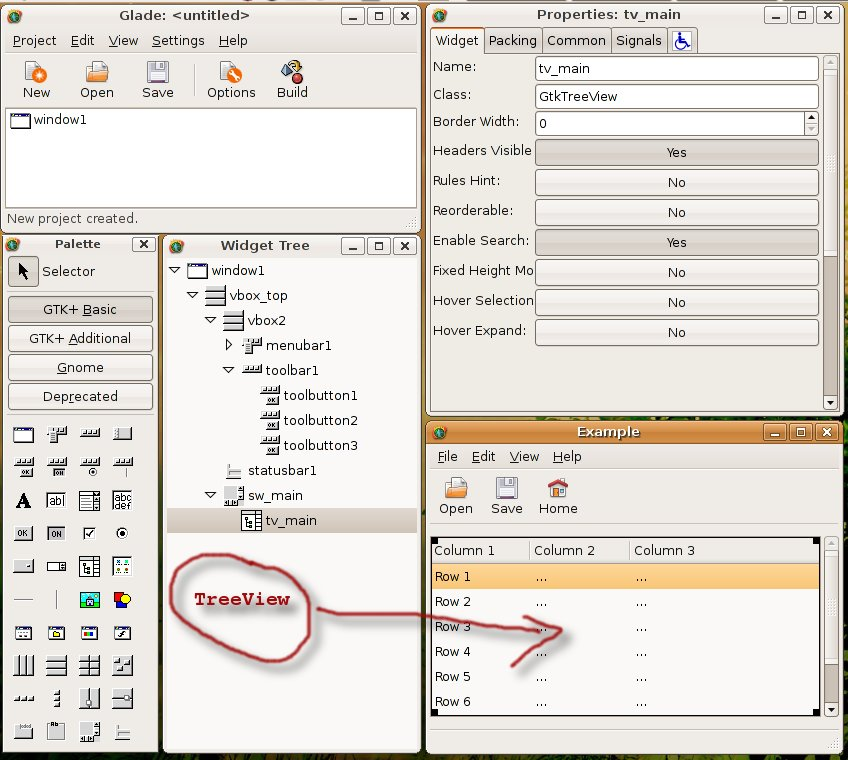
\includegraphics[width=12cm]{figs/png/treeview}
\caption{\label{fig:VR}Designing a \codename{TreeView} by means of \glade }
\end{center}
\end{figure}

In the example, the \codename{TreeView} has been called
\codename{tv\_main}, and after View creation the widget will be
available with that name.

{ \codesize 
\begin{verbatim}
from gtkmvc import View

class MyView (View):
  def __init__(self, controller):
    View.__init__(self, controller, 'test.glade')
    #...
    return
  pass 
\end{verbatim}
}

The \codename{ListStore} is of course not contained in the view, but
it is created and stored in the Model. If the model had to be also a
\codename{ListStore} (i.e.  derived from it) \codename{MyModel} had to
derive from \codename{gtkmvc.ListStoreModel} instead of
\codename{Model}. To keep things easier, Has--A relationship is
chosen.

{ \codesize 
\begin{verbatim}
from gtkmvc import Model
import gtk
import gobject

class MyModel (Model):
  def __init__(self):
    Model.__init__(self)

    self.list = gtk.ListStore(gobject.TYPE_INT, gobject.TYPE_STRING)
    return
  pass 
\end{verbatim}
}

The controller has the responsibility of connecting the
\codename{TreeView} and the \codename{ListStore}, and it creates
columns and renderers as well. Construction must occur after View has
been created. More precisely, the ideal time is during
view-registration.

{ \codesize 
\begin{verbatim}
from gtkmvc import Controller
import gtk

class MyCtrl (Controller):
  def __init__(self, m):
    Controller.__init__(self, m)
    return

  def register_view(self, view):
    Controller.__register_view(self, view)
    self.__setup_treeview()
    return

  def __setup_treeview(self):
    tv = self.view['tv_main']
    
    tv.set_model(self.model.list) # sets the model

    # creates the columns
    cell = gtk.CellRendererText()
    col = gtk.TreeViewColumn('Int', cell, text=0)
    tv.append_column(col)

    cell = gtk.CellRendererText()
    col = gtk.TreeViewColumn('String', cell, text=1)
    tv.append_column(col)

    # registers any treeview-related signals...

    return

  pass # end of class 
\end{verbatim}
}



\subsection{\label{OPD}Observable Properties in details}
The mechanism of the Observable Properties (\OP) is fully automatic,
since its management is carried out by the base class
\codename{Model}.

Basically the user derives from class \codename{Model} (or the others
listed in section \ref{MODELS}). The user and adds a class variable
called \OPvar. This variable must be a map, whose elements' keys are
names of properties, and the associated values are the initial values.

For example, suppose you want to create an \OP called \codename{name} 
initially associated to the string value ``Rob'':

{ \codesize 
\begin{verbatim} 
from gtkmvc import Model

class MyModel (Model):
  __properties__ = { 'name' : 'Rob' }

  def __init__(self):
    Model.__init__(self)
    # ...
    return

  pass # end of class
\end{verbatim}
}

By using a specific meta-class, property \codename{name} will be
automatically added, as well as all the code to handle it.

This means that you may use the property in this way:
{ \codesize 
\begin{verbatim} 
m = MyModel()
print m.name  # prints 'Rob'
m.name = 'Roberto' # changes the property value
\end{verbatim}
}

What's missing is now an observer, to be notified when the property
changes. To create an observer, derive your class from base class
\codename{gtkmvc.Observer}.

{ \codesize 
\begin{verbatim} 
from gtkmvc import Observer

class AnObserver (Observer):
  def __init__(self, model):
    Observer.__init__(self, model)

    # ...
    return

  def property_name_value_change(self, model, old, new):
    print ``Property name changed from '%s' to '%s''' % (old, new)
    return

  pass # end of class
\end{verbatim}
}

The Observer constructor gets an instance of a Model, and registers the
class instance itself to the given model, to become an observer of
that model instance.

To receive notifications for the property \codename{name}, the
observer must define a method called
\codename{property\_name\_value\_change} that when is automatically
called will get the instance of the model containing the changed
property, and the property's old and new values.

As already mentioned, when used in combination with the \mvc,
Controllers are also Observers of their models.

Here follows an example of usage:
{ \codesize 
\begin{verbatim} 
m = MyModel()
o = AnObserver(m)

print m.name  # prints 'Rob'
m.name = 'Roberto' # changes the property value, o is notified
\end{verbatim}
}

Things so far are easy enough, but they get a bit complicated when you
derive custom models from other custom models.  For example, what
happens to \OP if you derive a new model class from the class
\codename{MyModel}?

In this case the behavior of the \OP trusty follows the typical Object
Oriented rules:
\begin{enumerate}
    \item Any \OP in base class are inherited by derived classes.
    \item Derived class can override any \OP in base classes.
    \item If multiple base classes defines the same \OP, only the
      first \OP will be accessible from the derived class.
\end{enumerate}

For example:

{ \codesize
\begin{verbatim} 
from gtkmvc import Model

class Test1 (Model):
    __properties__ = {
        'prop1'  : 1
        }

    def __init__(self):
        Model.__init__(self)

        # this class is an observer of its own properties:
        self.register_observer(self) 
        return
    
    def property_prop1_value_change(self, model, old, new):
        print "prop1 changed from '%s' to '%s'" % (old, new)
        return
    pass # end of class

class Test2 (Test1):    
    __properties__ = {
        'prop2'  : 2,
        'prop1'  : 3
        }
    
    def __init__(self):
        Test1.__init__(self)
        
        # also this class is an observer of itself:
        self.register_observer(self)
        return
    
    def property_prop2_value_change(self, model, old, new):
        print "prop2 changed from '%s' to '%s'" % (old, new)
        return
    pass

# test code:
t1 = Test1()
t2 = Test2()

t2.prop2 = 20
t2.prop1 = 30
t1.prop1 = 10
\end{verbatim}
}

When executed, this script generates this output:
{ \codesize 
\begin{verbatim} 
prop2 changed from '2' to '20'
prop1 changed from '3' to '30'
prop1 changed from '1' to '10'
\end{verbatim}
}

As you can see, \codename{t2.prop1} overrides the \OP \codename{prop1}
defined in Test1 (they have different initial values).  Test2 could
also override method \codename{property\_prop1\_value\_change}:

{ \codesize 
\begin{verbatim} 
class Test2 (Test1):
  # ... copy from previous definition, and add:
   
  def property_prop1_value_change(self, model, old, new):
    print "Test2: prop1 changed from '%s' to '%s'" % (old, new)
    return   

  pass
\end{verbatim}
}

As you expect, the output in this case would be:
{ \codesize 
\begin{verbatim} 
prop2 changed from '2' to '20'
Test2: prop1 changed from '3' to '30'
prop1 changed from '1' to '10'
\end{verbatim}
}


\subsubsection{\label{KOBS:DET}Types of Observable Properties}

In section \ref{KOBS} we anticipated that there exist several types
of \OP. In the examples so far we have seen only \emph{value} \OPS,
meaning that observers will be notified of any change of \emph{value}
assigned to the corresponding \OP. What would happen if the value of
the property would be a complex object like a list, or a user-defined
class, and the object would change internally?

For example:

{ \codesize 
\begin{verbatim} 
from gtkmvc import Model

class MyModel (Model):
    __properties__ = {
        'prop1'  : [1,2,3]
        }

    def __init__(self):
        Model.__init__(self)
        ...
        return
    pass # end of class

m = MyModel()
m.prop1.append(4)
m.prop1[1] = 5
\end{verbatim}
}

Last two lines of the previous example actually change the \OP
internally, that is different from \emph{assigning} a new value to the
property like in \verb@m.prop1 = [5,4,3,2]@ that would trigger a value
notifications like those seen in previous examples.  Similar problem
is found when the property is assigned to a class instance, and then a
method that change the instance is called.

\emph{Mutable sequential types} and \emph{User classes} are also
supported by the \obs of \pygtkmvc, but the name of the notified
method in the controller has to be changed accordingly.
The idea is to provide two methods to be notified:
\begin{description}
\item[property\_\codename{name}\_before\_change] That is called
  immediately \emph{before} a method that changes the instance is
  called on the \OP called \codename{name}.
\item[property\_\codename{name}\_after\_change] That is called
  immediately \emph{after} a method that changes the instance is
  called on the \OP called \codename{name}.
\end{description}

Of course, it is not needed to define both of the two methods in the
observer class, as only the actually defined methods will be called. 

The signature of these methods is:
{ \codesize 
\begin{verbatim} 
    def property_<name>_before_change(self, model, instance, name,
                                      args, kwargs)

    def property_<name>_after_change(self, model, instance, name, 
                                     res, args, kwargs)
\end{verbatim}
}

\begin{description}
\item[self] The Observer class instance defining the method.
\item[model] The Model instance containing the \OP called
  \verb@<name>@ that is being changed.
\item[instance] The object instance that is assigned to the \OP called
  \verb@<name>@.
\item[name] The name of the method that is being called. This
  is different from \verb@<name>@ that is the name of the \OP
  contained in the model. 
\item[res] (Only for \emph{after} notification) the value returned by
  the method \emph{name} that has been called on the \OP
  \emph{instance}.
\item[args] List of arguments of the method \emph{name}.
\item[kwargs] Map of keyword arguments of the method \emph{name}.
\end{description}

As it can be noticed, the only difference between these two method
signatures is the parameter \emph{res} that is obviously available only
for notification method \emph{after}.

The framework \mvco provides a full support for python mutable
sequences like \kw{lists} and \emph{maps}. For example:


{ \codesize 
\begin{verbatim} 
from gtkmvc import Model, Observer

# ----------------------------------------------------------------------
class MyModel (Model):    
    __properties__ = {
        'myint'  : 0, 
        'mylist' : [],
        'mymap'  : {},
        }

    def __init__(self):
        Model.__init__(self)
        return    
    pass # end of class

# ----------------------------------------------------------------------
class MyObserver (Observer):
    def __init__(self, model):
        Observer.__init__(self, model)
        return

    # notifications

    def property_myint_value_change(self, model, old, new):
        print "myint changed"
        return

    def property_mylist_value_change(self, model, old, new):
        print "mylist changed"
        return

    def property_mylist_before_change(self, model, instance, name,
                                      args, kwargs):
        print "mylist before change:", instance, name, args, kwargs
        return

    def property_mylist_after_change(self, model, instance, name, res,
                                     args, kwargs):
        print "mylist after change:", instance, name, res, args, kwargs
        return

    # for mymap value_change and before_change are not provided!
    def property_mymap_after_change(self, model, instance, name, res,
                                    args, kwargs):
        print "mymap after change:", instance, name, res, args, kwargs
        return

    pass # end of class


# Look at what happens to the observer
if __name__ == "__main__":

    m = MyModel()
    c = MyObserver(m)

    # changes the int:
    m.myint = 20

    # changes the list:
    m.mylist = [1,2]             # calls value_change
    m.mylist.append(10)     
    m.mylist[0] = m.mylist[0]+1

    # changes the map:
    m.mymap["hello"] = 30
    m.mymap.update({'bye' : 50})
    del m.mymap["hello"]
    pass
\end{verbatim}
}

After the execution, this is the program output:

{ \codesize 
\begin{verbatim} 
myint changed
mylist changed
mylist before change: [1, 2] append (10,) {}
mylist after change: [1, 2, 10] append None (10,) {}
mylist before change: [1, 2, 10] __setitem__ (0, 2) {}
mylist after change: [2, 2, 10] None __setitem__ (0, 2) {}
mymap after change: {'hello': 30} None __setitem__ ('hello', 30) {}
mymap after change: {'bye': 50, 'hello': 30} update None ({'bye': 50},) {}
mymap after change: {'bye': 50} None __delitem__ ('hello',) {}
\end{verbatim}
}

This covers those cases where you have your \OPS holding mutable
sequence values. What if the value is a user-defined class instance?
The notification mechanism is the same: when a method \codename{M}
that changes internally the instance is called, Observer's methods
\kw{before} and \kw{after} will be called. However, how can the user
declare that method \codename{M} \emph{does changes} the instance?
Two mechanism are provided by the framework:
\begin{itemize}
\item For already existing classes and class instances. In this cases
  the declaration occurs when the instance is assigned to the \OP in
  the model.
\item For ad-hoc and new classes. In this case the method will be
  \emph{declared} as \kw{Observable} at the class level, through a
  special \kw{decorator} provided by the framework. This is the
  preferable manner. 
\end{itemize}

Examples for new classes:

{ \codesize 
\begin{verbatim} 
from gtkmvc import Model
from gtkmvc import Observer
from gtkmvc import observable

# ----------------------------------------------------------------------
class AdHocClass (observable.Observable):
    def __init__(self): self.val = 0

    # this way the method is declared as 'observed':
    @observable.observed 
    def change(self): self.val += 1

    # this is NOT observed:
    def is_val(self, val): return self.val == val

    pass #end of class

# ----------------------------------------------------------------------
class MyModel (Model):
    __properties__ = {
        'obj' : AdHocClass(),
        }

    def __init__(self):
        Model.__init__(self)
        return    

    pass # end of class

# ----------------------------------------------------------------------
class MyObserver (Observer):
    def __init__(self, model):
        Observer.__init__(self, model)
        return

    def property_obj_value_change(self, model, old, new):
        print "obj value changed from:", old, "to:", new 
        return

    def property_obj_after_change(self, model, instance, name, res,
                                  args, kwargs):
        print "obj after change:", instance, name, res, args, kwargs
        return

    pass

# Look at what happens to the observer
if __name__ == "__main__":
    m = MyModel()
    c = MyObserver(m)
    m.obj.change()
    m.obj = None
    pass
\end{verbatim}
}

The execution prints out (slightly modified for the sake of
readability):

{ \codesize 
\begin{verbatim} 
obj after change: <__main__.AdHocClass object at 0xb7d91e8c> 
change None (<__main__.AdHocClass object at 0xb7d91e8c>,) {}

obj value changed 
from: <__main__.AdHocClass object at 0xb7d91e8c> to: None
\end{verbatim}
}

As you can see, declaring a class as \emph{observable} is as simple as
deriving from \codename{gtkmvc.observable.Observable} and decorating
those class methods that must be observed with the decorator 
\codename{gtkmvc.observable.observe} (decorators are supported by
Python version 2.4 and later only). 

\vspace{4mm}
What if the user class cannot be easy changed, or only an instance of
the class is available as \OP value? In this case declaration of the
methods to be observed can be done at time of declaration of the
corresponding \OP. In this case the \emph{value} to be assigned to the
\OP must be a triple \verb@(class, instance, method_names>@, where:
\begin{description}
\item[class] Is the \codename{class} of the object to be observed.
\item[instance] Is the object to be observed.
\item[method\_names] Is a tuple of strings, representing the method
  names of the instance to be observed.
\end{description}

For example:
{ \codesize 
\begin{verbatim} 
from gtkmvc import Model

#----------------------------------------------------------------------
# This is a class the used cannot/don't want to change
class HolyClass (object):    
    def __init__(self): self.val = 0 
    def change(self): self.val += 1
    pass #end of class


# ----------------------------------------------------------------------
class MyModel (Model):

    __properties__ = {
        'obj' : (HolyClass, HolyClass(), ('change',)),
        }

    def __init__(self):
        Model.__init__(self)
        return    

    pass # end of class
\end{verbatim}
}



\vspace{4mm}
Finally, \OP can hold special values that are \kw{signals} that can be
used to notify observers that certain events occurred. 

To declare an \OP as a signal, the value of the \OP must be
\codename{gtkmvc.observable.Signal()}. To notify an event, the model
can then invoke method \codename{emit} of the \OP. The observers will
be notified by calling method
\codename{property\_<name>\_signal\_emit} that will also receive any
parameter passed to the \codename{emit} method. For example:

{ \codesize 
\begin{verbatim} 
from gtkmvc import Model
from gtkmvc import Observer
from gtkmvc import observable

# ----------------------------------------------------------------------
class MyModel (Model):
    __properties__ = {
        'sgn'  : observable.Signal(),
        }

    def __init__(self):
        Model.__init__(self)
        return    
    pass

# ----------------------------------------------------------------------
class MyObserver (Observer):
    def __init__(self, model):
        Observer.__init__(self, model)
        return

    # notification
    def property_sgn_signal_emit(self, model, args, kwargs):
        print "Signal:", model, args, kwargs
        return

    pass # end of class

# Look at what happens to the observer
if __name__ == "__main__":
    m = MyModel()
    c = MyObserver(m)
    m.sgn.emit() # we emit a signal
    m.sgn.emit("hello!", key=10) # with arguments
    pass
\end{verbatim}
}

The execution of this example will produce:

{ \codesize 
\begin{verbatim} 
Signal: <__main__.MyModel object at 0xb7de564c> () {}
Signal: <__main__.MyModel object at 0xb7de564c> ('hello!',) {'key': 10}
\end{verbatim}
}

In the \file{examples}, there are several examples that show how
different types of \OPS can be used. Of course all available types can
be used in all available kind of model classes, with or without
multi-threading support.

  
\subsubsection{Special members for Observable Properties}
Classes derived from Model, that exports \OPS, have several special
members. Advanced users might be interested can override some of them,
but in general they should be considered as private members. They are
explained here for the sake of completeness.

\begin{description}

\item[\OPvar] A class (static) member that maps property names and
initial values. This must be provided as a map by the user.

\item[\OPdvar] Automatically generated static member that maps the 
\OPS exported by all base classes. This does not contain \OPS that 
the class overrides. 

\item[\codename{\_prop\_\emph{property\_name}}] This is an
  auto-generated variable to hold the property value. For example, a
  property called \codename{x} will generate a variable called
  \codename{\_prop\_x}.

\item[\codename{get\_prop\_\emph{property\_name}}] This public method
  is the getter for the property. It is automatically generated only
  if the user does not define one. This means that the user can change
  the behavior of it by defining their own method.  For example, for
  property \codename{x} the method is \codename{get\_prop\_x}.  This
  method gets only self and returns the corresponding property value.

\item[\codename{set\_prop\_\emph{property\_name}}] This public method
  is customizable like \\
  \codename{get\_prop\_<property\_name>}.  This does not return
  anything, and gets self and the value to be assigned to the
  property. The default auto-generated code also calls method
  \codename{gtkmvc.Model.notify\_property\_change} to notify the
  change to all registered observers.

\end{description}

For further details about this topic see meta-classes \codename{PropertyMeta}
and \\
\codename{ObservablePropertyMeta} from package \codename{support}.


